\documentclass[11pt,letterpaper]{article}
\usepackage[utf8]{inputenc}

%----- Configuración del estilo del documento------%
\usepackage[table]{xcolor}
\usepackage{epsfig,graphicx}
\usepackage[left=2cm,right=2cm,top=1.8cm,bottom=2.3cm]{geometry}
\usepackage{fancyhdr}
\usepackage{lastpage}
\pagestyle{fancy}
\fancyhf{}
\rfoot{\textit{Página \thepage \hspace{1pt} de \pageref{LastPage}}}


%------ Paquetes matemáticos básicos --------%
\usepackage{amsmath}
\usepackage{amssymb}
\usepackage{amsthm}

%------ Texto aleatorio ----- %

\usepackage{lipsum}



\begin{document}

%------ Encabezado -------- %

\begin{center}
    \begin{minipage}{3cm}
    	\begin{center}
    		\includegraphics[height=3.4cm]{./imagenes/logo_unam.png}
    	\end{center}
    \end{minipage}\hfill
    \begin{minipage}{10cm}
    	\begin{center}
    	\textbf{\large Universidad Nacional Autónoma de México}\\[0.1cm]
        \textbf{Facultad de Ciencias}\\[0.1cm]
        \textbf{Estructuras Discretas $|$ Grupo 7020}\\[0.1cm]
        \textbf{Tarea 2: Lógica Preposicional}\\[0.1cm]
        Real Araiza Yamile\\[0.1cm]
        Rodríguez López Luis Fernando\\[0.1cm]
        Tenorio Reyes Ihebel Luro\\[0.1cm]
        27/09/2024
    	\end{center}
    \end{minipage}\hfill
    \begin{minipage}{3cm}
    	\begin{center}
    		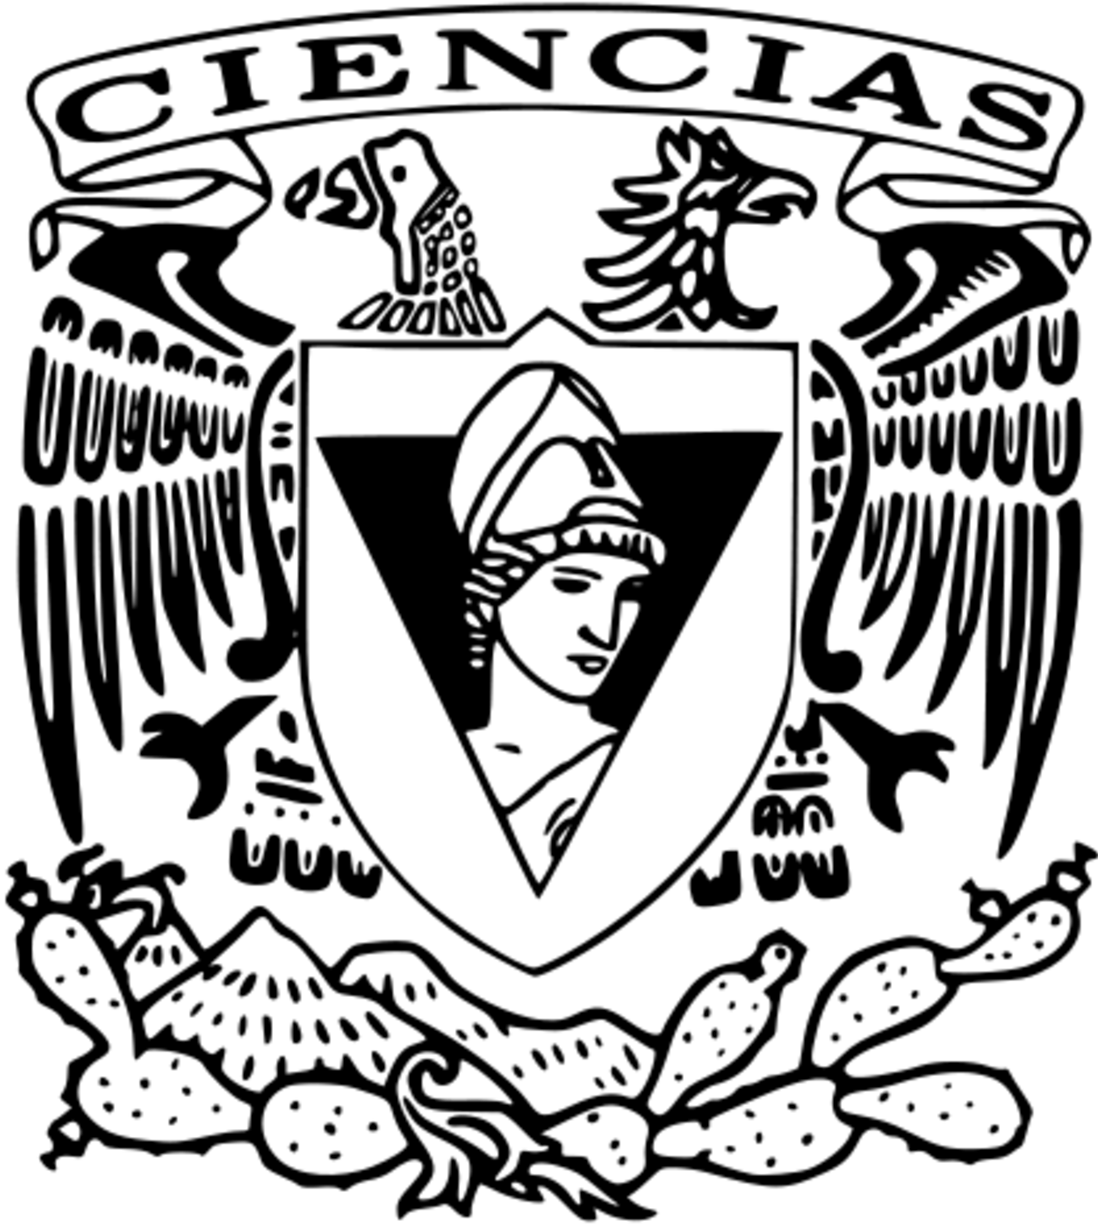
\includegraphics[height=3.4cm]{./imagenes/Logo_FC.png}
    	\end{center}
    \end{minipage}
\end{center}

\rule{17cm}{0.1mm}

%------ Fin de encabezado -------- %

\section*{Indicaciones}

%------ Ejercicio 01 ------%

\section*{Construcción de una montaña rusa sección 3.1 del Stewart }
Suponga que se le solicita que diseñe el primer ascenso y descenso de una nueva montaña rusa. Después de estudiar fotografías de sus montañas rusas predilectas, decide hacer la pendiente de ascenso 0.8 y la de descenso -1.6. Opta por conectar estos dos tramos rectos $y=L_1(x)$ y $y=L_2(x)$ mediante parte de una parábola $y=f(x)=ax^2+bx+c$, donde $x$ y $f(x)$ se miden en pies. Para que el trayecto sea uniforme, no pueden existir cambios abruptos de dirección, por lo que se desea que el trayecto sea uniforme, no pueden existir cambios abruptos de dirección, por lo que se desea que los segmentos de recta $L_1$ y $L_2$ sean tangentes a la parábola en los puntos de transición P y Q.
Para simplificar las ecuaciones, decide situar el origen en P.

\subsection*{Parte 1.}
\subsubsection*{a) Suponga que la distancia horizontal entre P y Q es 100 pies. Escriba ecuaciones en a, b y c que aseguren que el trayecto sea suave en los puntos de transición}
Sabemos que la curva f(x) debe ser tangente a $L_1$ y $L_2$, por lo que necesitamos su derivada.
\begin{equation*}
  f'(x)=2ax+b
\end{equation*}
De aquí, podemos decir que f'(x) evaluada en 0 y 100 (por la distancia horizontal de 100ft) debe dar 4/5 y -8/5 respectivamente, para C, sabemos que es equivalente a la posición vertical vértice de f, es decir, el punto más alto, donde la pendiente tangente es igual a 0
\begin{equation*}
  \begin{split}
    2ax+b &= 0 \\
    2ax &= b \\
    x &= \frac{b}{2a}
  \end{split}
\end{equation*}
Y para obtener c, igualamos $ax²+by+c$ con 0 y lo evaluamos al mismo tiempo con 0, esto por que sabemos que pasa por el punto (0,0) \\
\begin{equation*}
  \begin{split}
    \textbf{Ec. 1. } & 2a(0)+b \ = \ \frac{4}{5} \\
    \textbf{Ec. 2. } & 2a(100)+b \ = \ -\frac{8}{5} \\
    \textbf{Ec. 3. } & a(0)^2+b(0)+c=0
  \end{split}
\end{equation*}
\subsubsection*{b) Resuelva las ecuaciones del inciso a para a, b y c para hallar una fórmula para f(x)}
\textbf{Ec. 1.} \\
\begin{equation*}
  \begin{split}
    2a(0)+b &= \frac{4}{5} \\
    b &= \frac{4}{5}
  \end{split}
\end{equation*}
\textbf{Ec. 2.} \\
\begin{equation*}
  \begin{split}
    2a(100)+b &= -\frac{8}{5} \\
    2a(100) &= -\frac{8}{5}-\underbrace{b}_{\text{Sustituimos}} \\
    200a &= -\frac{8}{5}-\frac{4}{5} \\
    a &= -\frac{12}{5\cdot200} \\
    a &= -\frac{3}{250}
  \end{split}
\end{equation*}
\textbf{Ec. 3.} \\
Sustiumos en f(0)=0 para obtener c.
\begin{equation*}
  \begin{split}
    -\frac{3}{250}(0)^2+\frac{4}{5}(0)+c &= 0 \\
    c &= 0
  \end{split}
\end{equation*}
$\therefore$ podemos concluir que $f(x)$ está dada por:
\begin{equation*}
  f(x)=-\frac{3}{250}x^2+\frac{4}{5}b
\end{equation*}
\subsubsection*{c) Dibuje $L_1$, $f(x)$ y $L_2$ para verificar gráficamente que las transiciones sean suaves.}
tenemos f(x) pero necesitamos obtener $L_1$ y $L_2$. \\
\textbf{Ec. $L_1(x)$.} \\
De la forma de la recta y=mx+b, tenemos que m = 4/5 y como la intersección en el eje \textit{y} es en 0, b = 0. \\
$\therefore L_1(x)=\frac{4}{5}x$. \\
\textbf{Ec. $L_2(x)$.}\\
Necesitamos un un punto por el que pase $L_2$, y sabemos que tiene un punto que coincide con f(x) cuando x está evaluado en 100, por tanto, resolvemos f(100).
\begin{equation*}
  \begin{split}
    f(100) &= \underbrace{-\frac{3}{250}(100)^2+\frac{4}{5}(100)}_{\text{Resolviendo con calculadora.}} \\
    f(100) &= -40
  \end{split}
\end{equation*}
Ahora teniendo el punto (100,-40) que es Q, utilizamos la fórmula punto pendiente para obtener $L_2$.
\begin{equation*}
  \begin{split}
    y+40 &= -\frac{8}{5}(x-100) \\
    y+40 &= -\frac{8}{5}x+8(20) \\
    y &= -\frac{8}{5}x+160-40 \\
    y &= -\frac{8}{5}x+120
  \end{split}
\end{equation*}
$\therefore L_2(x)=-\frac{8}{5}x+120$. \\
\textbf{Graficando $L_1$, $f(x)$ y $L_2$ con geogebra:}
\begin{center}
  \includegraphics[width=15cm]{./imagenes/montañarusa1.png}
\end{center}

\subsubsection*{d) Encuentre la diferencia en la elevación entre P y Q}
Sabemos que P está en el punto (0,0) y Q en (100,-40). \\
$\therefore$ La diferencia de altura es de 40ft
\subsection{Parte 2.}
La solución del problema 1 puede \textit{parecer} suave, pero es posible que no \textit{sienta} lo suave debido a que la pieza definida como función [consistente en $L_1(x)$ para x<0, $f(x)$ para 0 $\leq$ x $\leq$ 100; y $L_2(x)$ para x>100] no tiene una segunda derivada contínua. Por consiguiente, usted decide mejorar su diseño utilizando una función cuadrática $q(x)=ax^2+bx+c$ únicamente en el intervalo 10 $\leq$ x $\leq$ 90 y conectarlo con las funciones lineales por medio de dos funciones cúbicas:
\begin{equation*}
  \begin{split}
    g(x)=kx^3+lx^2+mx+n  &\text{  Para: } 0 \leq x < 10 \\
    h(x)=px^3+qx^2+rx+s  &\text{  Para: } 90 \leq x < 100
  \end{split}
\end{equation*}
\subsubsection*{a) Escriba un sistema de ecuaciones con 11 incógnitas que aseguren que las funciones y sus dos primeras derivadas coincidan en los puntos de transición.}
\begin{equation*}
  \begin{split}
    \textbf{Ec. 1 } & L_1(0)=g(0) \\
    \textbf{Ec. 2 } & g(10)=q(10) \\
    \textbf{Ec. 3 } & q(90)=h(90) \\
    \textbf{Ec. 4 } & h(100)=L(100) \\
    \textbf{Ec. 5 } & L_1'(0)=g'(0) \\
    \textbf{Ec. 6 } & g'(10)=q'(10) \\
    \textbf{Ec. 7 } & q'(90)=h'(90) \\
    \textbf{Ec. 8 } & h'(100)=L'(100) \\
    \textbf{Ec. 9 } & L_1(0)=g(0) \\
    \textbf{Ec. 10 } & g(10)=q(10) \\
    \textbf{Ec. 11 } & q(90)=h(90) \\
    \textbf{Ec. 12 } & h(100)=L(100)
  \end{split}
\end{equation*}
De aquí, obtenemos primero las derivadas y segundas derivadas de todas las ecuaciones.
\begin{equation*}
  \begin{split}
    L_1(x) &= \frac{4}{5}x \\
    L_1'(x) &= \frac{4}{5} \\
    L_1''(x) &= 0 \\
    g(x) &= kx^3+lx^2+mx+n \\
    g'(x) &= 3kx^2+2lx+m \\
    g''(x) &= 6kx+2l \\
    q(x) &= ax^2+bx+c \\
    q'(x) &= 2ax+b \\
    q''(x) &= 2a \\
    h(x) &= px^3+qx^2+rx+s \\
    h'(x) &= 3px^2+2qx+r \\
    h''(x) &= 6px+2q \\
    L_2(x) &= -\frac{8}{5}x+120 \\
    L_2'(x) &= -\frac{8}{5} \\
    L_2''(x) &= 0
  \end{split}
\end{equation*}
De aquí, sustituyendo las funciones en el sistema de ecuaciones y evaluando x en sus respectivos puntos, tenemos el siguiente sistema de ecuaciones de 11 incognitas.
\begin{equation}
\begin{split}
  1000k + 100l + 10m + n &= 100a + 10b + c \\
  300k + 20l + m &= 20a + b \\
  60k + 2l &= 2a \\
  30k + l &= a \\
  729000p + 8100q + 90r + s &= 8100a + 90b + c \\
  24300p + 180q + r &= 180a + b \\
  540p + 2q &= 2a \\
  270p + q &= a \\
  n &= 0 \\
  m &= \frac{4}{5} \\
  l &= 0 \\
  1000000p + 10000q + 100r + s &= -40 \\
  30000p + 200q + r &= -\frac{8}{5} \\
  300p + q &= 0
\end{split}
\end{equation}

\subsubsection*{b) Resuelva las ecuaciones del inciso a) con un sistema algebráico computarizado para encontrar las fórmulas para q(x), g(x) y h(x).}
Utilizando python:
\begin{verbatim}
from sympy import symbols, Eq, solve
# Definir las incógnitas
a, b, c, k, l, m, n, p, q, r, s = symbols('a b c k l m n p q r s')
# Ecuaciones según las condiciones dadas
eq1 = Eq(1000*k + 100*l + 10*m + n, 100*a + 10*b + c)
eq2 = Eq(300*k + 20*l + m, 20*a + b)
eq3 = Eq(60*k + 2*l, 2*a)
eq4 = Eq(30*k + l, a)
eq5 = Eq(729000*p + 8100*q + 90*r + s, 8100*a + 90*b + c)
eq6 = Eq(24300*p + 180*q + r, 180*a + b)
eq7 = Eq(540*p + 2*q, 2*a)
eq8 = Eq(270*p + q, a)
eq9 = Eq(n, 0)
eq10 = Eq(m, 4/5)
eq11 = Eq(l, 0)
eq12 = Eq(1000000*p + 10000*q + 100*r + s, -40)
eq13 = Eq(30000*p + 200*q + r, -8/5)
eq14 = Eq(300*p + q, 0)# Resolver el sistema de ecuaciones
solution = solve((eq1, eq2, eq3, eq4, eq5, eq6, eq7, eq8, eq9, eq10, eq11, eq12, eq13, ...
 eq14), (a, b, c, k, l, m, n, p, q, r, s))
# Mostrar la solución
solution
\end{verbatim}
que nos arroja:
\begin{verbatim}
{a: -0.0133333333333333,
 b: 0.933333333333333,
 c: -0.444444444444444,
 k: -0.000444444444444444,
 l: 0.0,
 m: 0.800000000000000,
 n: 0.0,
 p: 0.000444444444444444,
 q: -0.133333333333333,
 r: 11.7333333333333,
 s: -324.444444444444}
\end{verbatim}
Que sustituyendo en las funciones g(x), q(x) y h(x) nos da:
\begin{equation*}
  \begin{split}
    g(x)=-0.000444x^3+0.8x &\text{  cuando  } 10 \leq x < 10 \\
    h(x)=0.000444x^3-0.133x^2+11.7333x-324.4444 &\text{  cuando  } 90 \leq x < 100 \\
    q(x) = -0.0133x^2+0.9333x-0.4444 &\text{  cuando  } 10 \leq x < 90
  \end{split}
\end{equation*}
\subsubsection*{c) Dibuje $L_1$, $g(x)$, $q(x)$, $h(x)$ y $L_2(x)$ y comparelos con las gráficas del problema 1 inciso c).}
\textbf{Graficando $L_1$, $f(x)$ y $L_2$ con geogebra:}
\begin{center}
  \includegraphics[width=15cm]{./imagenes/montañarusa2.png}
\end{center}
Aunque a simple vista se vean muy parecidos, es notorio el suavizado que hacen las funciones auxiliares de forma que es muy poco abrupta la transición de ir en linea recta a nuestro ascenso y descenso diseñados para llegar a la segunda recta.

%------ Ejercicio 02 ------%
\section*{¿Dónde debería un piloto iniciar el aterrizaje? sección 3.4 del Stewart }
%------ Ejercicio 03 ------%
\section*{Ejercicio 80 sección 3.5 del Stewart}

En la figura se muestra una lámpara colocada tres unidades hacia la derecha del eje \( y \) y una sombra creada por la región elíptica \( x^2 + 4y^2 \leq 5 \). Si el punto \( (-5, 0) \) está en el borde de la sombra, ¿qué tan arriba del eje \( x \) está colocada la lámpara?

\begin{center}
    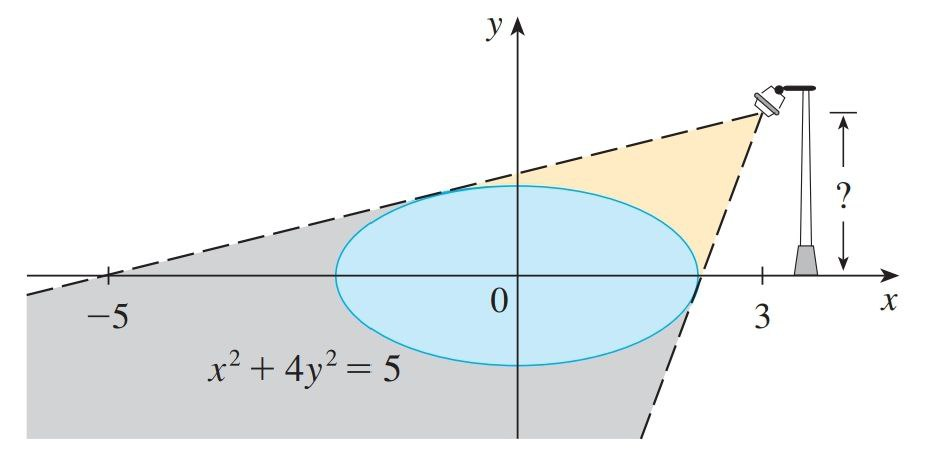
\includegraphics[height=7.0cm]{./imagenes/lampara.jpg}
\end{center}

Se nos da la ecuación de una elipse:

\[
x^2 + 4y^2 = 5
\]

Una lámpara está colocada en el punto \( (3, h) \) y un punto de intersección de la sombra proyectada se encuentra en \( (-5, 0) \). Nuestro objetivo es encontrar el valor de \(h\).

\subsection{Paso 1: Ecuación de la recta que conecta los puntos}

La pendiente \(m\) de la recta que pasa por los puntos \( (-5, 0) \) y \( (3, h) \) es:

\[
m = \frac{h - 0}{3 - (-5)} = \frac{h}{8}
\]

Por lo tanto, la ecuación de la recta que conecta estos dos puntos es:

\[
y = \frac{h}{8}(x + 5)
\]

\subsection*{Paso 2: Sustitución en la ecuación de la elipse}

Sabemos que la recta debe intersectar la elipse, por lo que sustituimos la ecuación de la recta \( y = \frac{h}{8}(x + 5) \) en la ecuación de la elipse \( x^2 + 4y^2 = 5 \):

\[
x^2 + 4\left( \frac{h}{8}(x + 5) \right)^2 = 5
\]

Expandiendo el término al cuadrado:

\[
x^2 + 4\left( \frac{h^2}{64}(x + 5)^2 \right) = 5
\]

Simplificando:

\[
x^2 + \frac{h^2}{16}(x^2 + 10x + 25) = 5
\]

Multiplicamos ambos lados de la ecuación por 16 para eliminar los denominadores:

\[
16x^2 + h^2(x^2 + 10x + 25) = 80
\]

\subsection*{Paso 3: Resolver para \(h\)}

Para resolver \(h\), usamos el hecho de que la recta debe intersectar la elipse. Elegimos el punto \(x = 0\) para simplificar el cálculo. Sustituyendo \(x = 0\) en la ecuación:

\[
16(0)^2 + h^2(0^2 + 10(0) + 25) = 80
\]

Simplificando:

\[
25h^2 = 80
\]

Despejando \(h\):

\[
h^2 = \frac{80}{25} = 3.2
\]

Por lo tanto, la altura \(h\) es:

\[
h = \sqrt{3.2} \approx 1.79
\]

\subsection*{Conclusión}

La lámpara está colocada aproximadamente a una altura de \(h \approx 1.79\) unidades sobre el eje \(x\).

%------ Ejercicio 04 ------%
\section*{Ejercicio 40 sección 3.1 del Anton-Bivens-Davis}

Utilice una herramienta de gráficos para generar los gráficos de f' y f'' sobre el intervalo indicado: luegoutilice esos gráficos para estimar las coordenadas x de los puntos de inflexión de f, los intervalos en los que es cóncava hacia arriba o hacia abajo y los intervalos en los que f aumenta o disminuye. Verifique sus estimaciones graficando f.

\subsection*{Función y Derivadas}

Consideramos la función:

\[
f(x) = \frac{1}{1+x^2} \quad \text{en el intervalo} \quad -5 \leq x \leq 5.
\]

\subsubsection*{Primera Derivada}

La primera derivada de \( f(x) \) es:

\[
f'(x) = \frac{(1+x^2) \cdot 0 - 1 \cdot (2x)}{(1+x^2)^2} = \frac{-2x}{(1+x^2)^2}.
\]

\subsubsection*{Segunda Derivada}

La segunda derivada de \( f(x) \) es:

\[
f''(x) = \frac{(1+x^2)^2 \cdot (0) - (-2x) \cdot (2(1+x^2)(2x))}{(1+x^2)^4} = \frac{6x^2 - 2}{(1+x^2)^3}.
\]

\begin{center}
    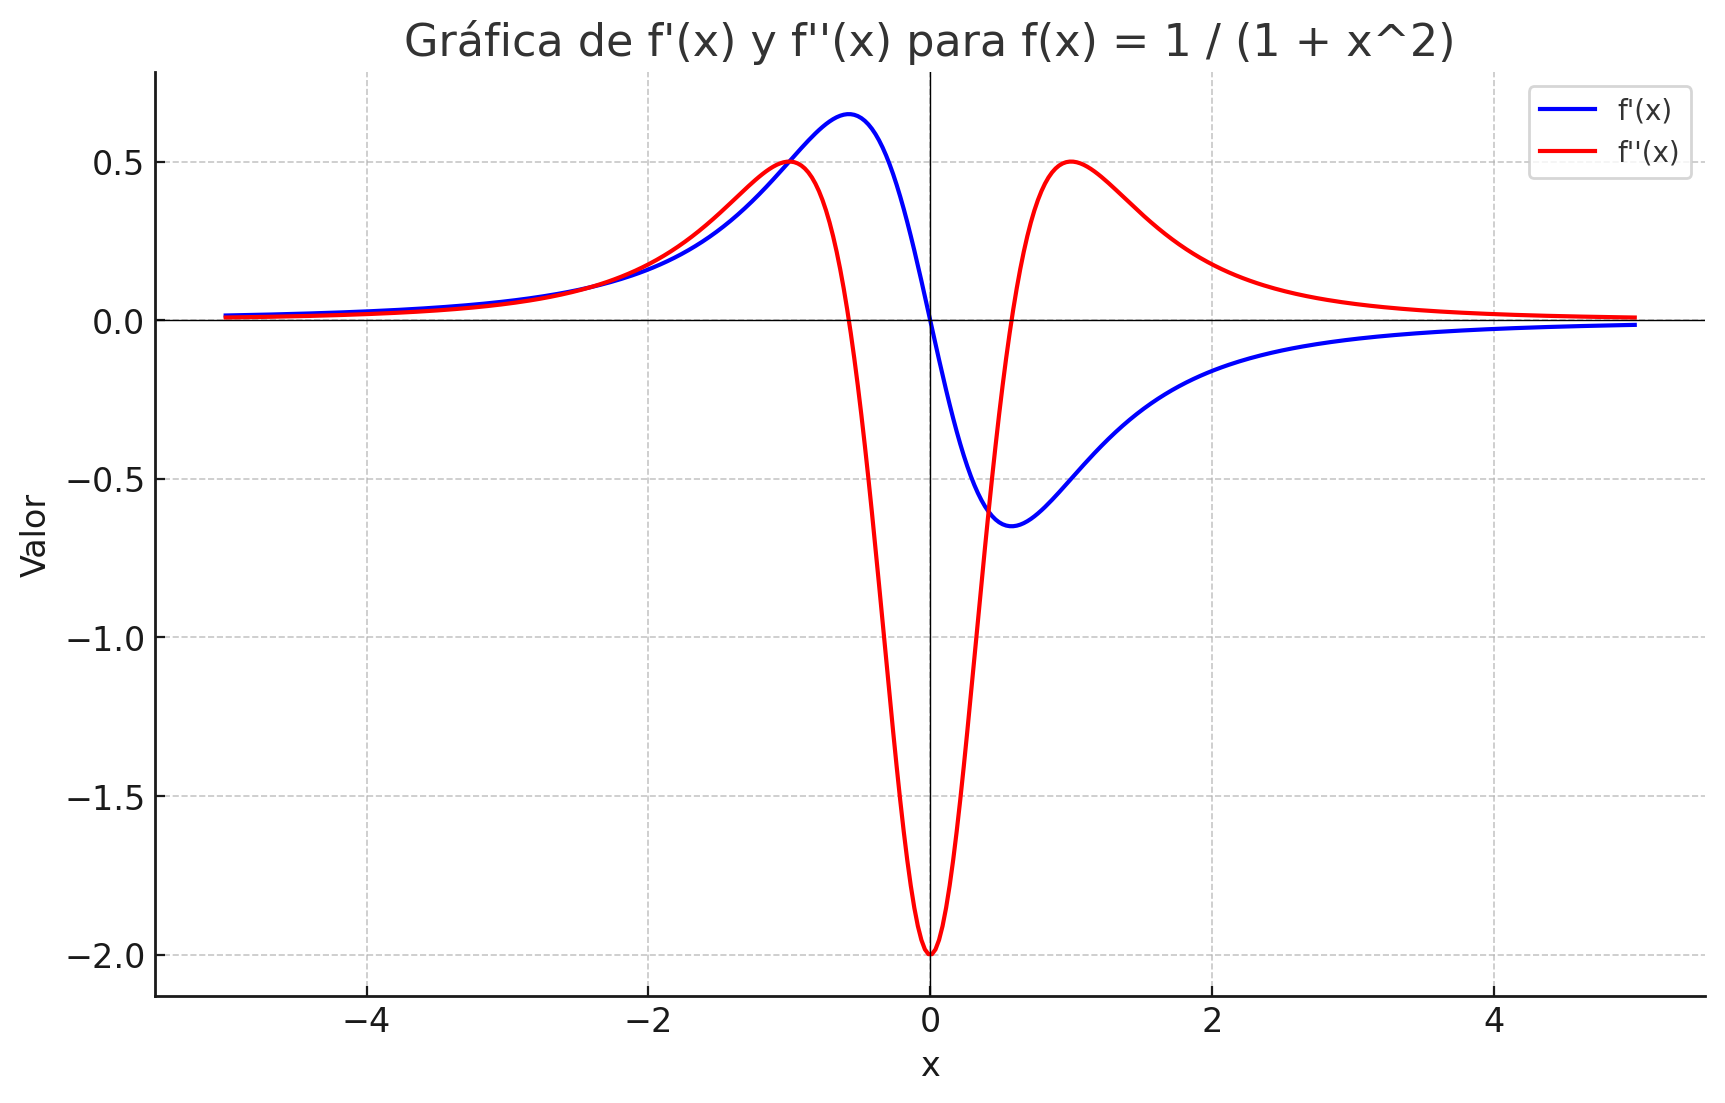
\includegraphics[width=17cm]{./imagenes/grafica1.png}
\end{center}

Aquí tienes la gráfica de las derivadas primera \( f'(x) \) (en azul) y segunda \( f''(x) \) (en rojo) de la función \( f(x) = \frac{1}{1+x^2} \) en el intervalo \( -5 \leq x \leq 5 \).

\begin{itemize}
    \item \( f'(x) \) muestra los intervalos donde la función es creciente o decreciente.
    \item \( f''(x) \) permite identificar los puntos de inflexión y la concavidad de la función.
\end{itemize}

Puedes observar cómo \( f'(x) = 0 \) en \( x = 0 \), y cómo \( f''(x) \) cambia de signo en los puntos de inflexión \( x = \pm \sqrt{3} \).

A partir de los gráficos de \( f'(x) \) (azul) y \( f''(x) \) (rojo), podemos hacer las siguientes estimaciones:

\subsection*{1. Puntos de inflexión:}

Los puntos de inflexión ocurren cuando la derivada segunda \( f''(x) \) cambia de signo. Observando la gráfica roja de \( f''(x) \), parece que cambia de signo alrededor de \( x \approx \pm 0.577 \), lo cual coincide con la fórmula teórica de los puntos de inflexión para \( f(x) = \frac{1}{1 + x^2} \).

Entonces, los puntos de inflexión son aproximadamente:
\[
x \approx \pm 0.577
\]

\subsection*{2. Concavidad:}

\begin{itemize}
    \item \textbf{Cóncava hacia arriba:} La función \( f(x) \) es cóncava hacia arriba cuando \( f''(x) > 0 \). Observamos en la gráfica que \( f''(x) \) es positiva cuando \( |x| > 0.577 \). Así que la función es cóncava hacia arriba en los intervalos:
    \[
    (-\infty, -0.577) \cup (0.577, \infty)
    \]
    
    \item \textbf{Cóncava hacia abajo:} \( f(x) \) es cóncava hacia abajo cuando \( f''(x) < 0 \). Esto ocurre en el intervalo donde \( |x| < 0.577 \), es decir:
    \[
    (-0.577, 0.577)
    \]
\end{itemize}

\subsection*{3. Crecimiento y decrecimiento:}

\begin{itemize}
    \item \textbf{Crecimiento:} La función \( f(x) \) es creciente cuando \( f'(x) > 0 \). En la gráfica verde, vemos que esto ocurre para \( x < 0 \), lo que indica que la función es creciente en el intervalo:
    \[
    (-5, 0)
    \]
    
    \item \textbf{Decrecimiento:} La función \( f(x) \) es decreciente cuando \( f'(x) < 0 \). En la gráfica verde, esto ocurre para \( x > 0 \), lo que indica que la función es decreciente en el intervalo:
    \[
    (0, 5)
    \]
\end{itemize}

\subsection*{Resumen:}

\begin{itemize}
    \item \textbf{Puntos de inflexión:} \( x \approx \pm 0.577 \).
    \item \textbf{Concavidad:}
    \begin{itemize}
        \item Cóncava hacia arriba en \( (-\infty, -0.577) \cup (0.577, \infty) \).
        \item Cóncava hacia abajo en \( (-0.577, 0.577) \).
    \end{itemize}
    \item \textbf{Crecimiento:} \( (-5, 0) \).
    \item \textbf{Decrecimiento:} \( (0, 5) \).
\end{itemize}

\begin{center}
    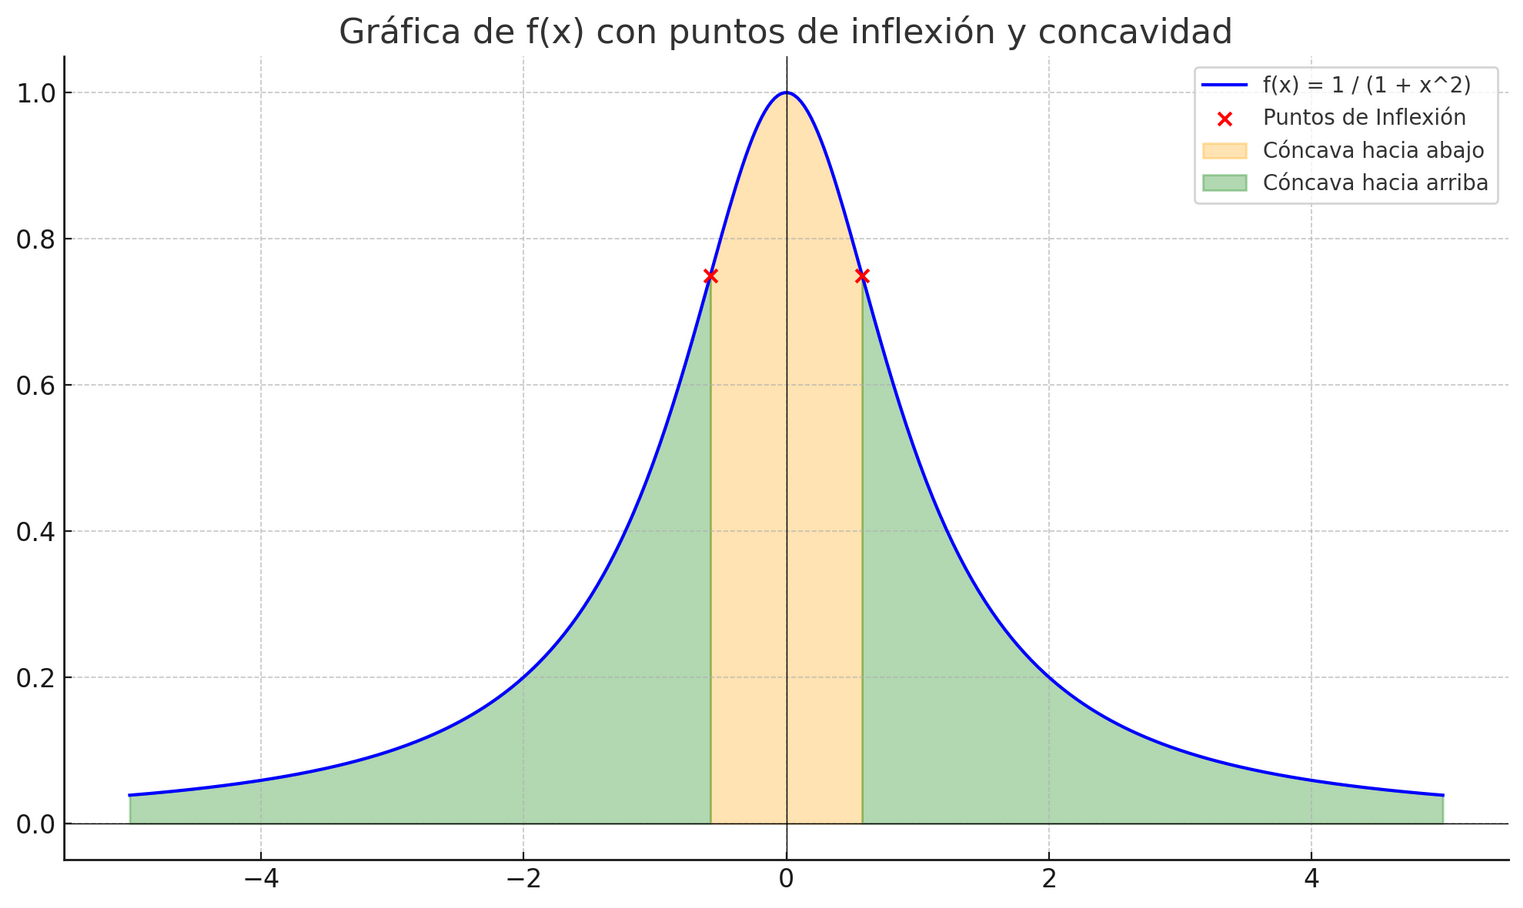
\includegraphics[width=17cm]{./imagenes/grafica.png}
\end{center}

%------ Ejercicio 05 ------%
\section*{Ejercicio 16 sección 3.7 del Stewart}
%------ Ejercicio 06 ------%
\section*{Ejercicio 19 sección 3.7 del Stewart}
La cantidad de carga, Q, en coulombs c) que ha pasado por un punto de un alambre hasta el tiempo t (medido en segundos) se expresa con Q(t) = t³ -2t² +6t +2. Encuentre la corriente cuando a)t = 0.5 s y b)t = 1 s. [Véase el ejemplo 3. La unidad de corriente es el ampere
(1A = 1C/s)]. ¿En qué momento la corriente es la más baja?

La cantidad de carga \( Q(t) \), en coulombs, que ha pasado por un punto de un alambre hasta el tiempo \( t \) (medido en segundos) está dada por la ecuación:

\[
Q(t) = t^3 - 2t^2 + 6t + 2
\]

Debemos encontrar la corriente cuando:

\begin{itemize}
    \item[a)] \( t = 0.5 \, \text{s} \)
    \item[b)] \( t = 1 \, \text{s} \)
\end{itemize}

\subsection*{Paso 1: Derivada de la carga con respecto al tiempo}

La corriente \( I(t) \) es la derivada de la carga \( Q(t) \) con respecto al tiempo \( t \):

\[
I(t) = \frac{dQ(t)}{dt}
\]

Primero, derivamos la función \( Q(t) \):

\[
\frac{d}{dt} \left( t^3 - 2t^2 + 6t + 2 \right) = 3t^2 - 4t + 6
\]

Por lo tanto, la corriente en función del tiempo es:

\[
I(t) = 3t^2 - 4t + 6
\]

\subsection*{Paso 2: Sustitución de valores}

\begin{itemize}
    \item[a)] Para \( t = 0.5 \, \text{s} \):

    \[
    I(0.5) = 3(0.5)^2 - 4(0.5) + 6 = 3(0.25) - 2 + 6 = 0.75 - 2 + 6 = 4.75 \, \text{A}
    \]

    \item[b)] Para \( t = 1 \, \text{s} \):

    \[
    I(1) = 3(1)^2 - 4(1) + 6 = 3(1) - 4 + 6 = 3 - 4 + 6 = 5 \, \text{A}
    \]
\end{itemize}

\subsection*{Respuesta}

\begin{itemize}
    \item La corriente cuando \( t = 0.5 \, \text{s} \) es \( 4.75 \, \text{A} \).
    \item La corriente cuando \( t = 1 \, \text{s} \) es \( 5 \, \text{A} \).
\end{itemize}

\subsection*{Encontrar el momento en que la corriente es más baja}

Para encontrar el momento en que la corriente es más baja, necesitamos encontrar el mínimo de la función de corriente \( I(t) = 3t^2 - 4t + 6 \).

\subsection*{Paso 1: Derivar la función de corriente}

Primero, derivamos \( I(t) \) con respecto al tiempo \( t \) para encontrar los puntos críticos:

\[
\frac{dI(t)}{dt} = 6t - 4
\]

\subsection*{Paso 2: Encontrar los puntos críticos}

Igualamos la derivada a cero para encontrar el valor de \( t \) en el cual la corriente puede ser mínima:

\[
6t - 4 = 0
\]

\[
6t = 4
\]

\[
t = \frac{4}{6} = \frac{2}{3} \, \text{s}
\]

\subsection*{Paso 3: Verificación}

Para asegurarnos de que este es un mínimo, podemos evaluar la concavidad usando la segunda derivada:

\[
\frac{d^2I(t)}{dt^2} = 6
\]

Como la segunda derivada es positiva (\( 6 > 0 \)), la función es cóncava hacia arriba, lo que confirma que \( t = \frac{2}{3} \, \text{s} \) es un mínimo.

\subsection*{Respuesta}

La corriente es más baja en \( t = \frac{2}{3} \, \text{s} \).

%------ Ejercicio 06 ------%
\section*{Ejercicio 21 sección 3.7 del Stewart}




\end{document}
